\documentclass[11pt,twoside]{book}

%%Page Size (rev. 08/19/2016)
%\usepackage[inner=0.5in, outer=0.5in, top=0.5in, bottom=0.5in, papersize={6in,9in}, head=12pt, headheight=30pt, headsep=5pt]{geometry}
\usepackage[inner=0.5in, outer=0.5in, top=0.5in, bottom=0.5in, papersize={5.5in,8.5in}, head=12pt, headheight=30pt, headsep=5pt]{geometry}
%% width of textblock = 324 pt / 4.5in
%% A5 = 5.8 x 8.3 inches -- if papersize is A5, then margins should be [inner=0.75in, outer=0.55in, top=0.4in, bottom=0.4in]


%%Header (rev. 4/11/2011)
\usepackage{fancyhdr}
 \pagestyle{fancy}
\renewcommand{\chaptermark}[1]{\markboth{#1}{}}
\renewcommand{\sectionmark}[1]{\markright{#1}}
 \fancyhf{}
\fancyhead[LE,RO]{\thepage}
\fancyhead[CE]{\leftmark}
\fancyhead[CO]{\rightmark}
 \fancypagestyle{plain}{ %
\fancyhf{} % remove everything
\renewcommand{\headrulewidth}{0pt} % remove lines as well
\renewcommand{\footrulewidth}{0pt}}



\usepackage[autocompile,allowdeprecated=false]{gregoriotex}
\usepackage{gregoriosyms}
\gresetgregoriofont[op]{greciliae}




%%Titles (rev. 9/4/2011) -- TOCLESS --- lets you have sections that don't appear in the table of contents

\setcounter{secnumdepth}{-1}

\usepackage[compact,nobottomtitles*]{titlesec}
\titlespacing*{\chapter}{0pt}{-30pt}{0pt}
\titlespacing*{\section}{0pt}{*0}{*1}
\titlespacing*{\subsubsection}{0pt}{*0}{*0}
\titlespacing*{\subsubsubsection}{0pt}{10pt}{*0}
\titleformat{\part} {\normalfont\Huge\sc\center}{\thechapter}{1em}{}
\titleformat{\chapter} {\normalfont\LARGE\sc\center}{\thechapter}{1em}{}
\titleformat{\section} {\normalfont\Large\sc\center}{\thesection}{1em}{}
\titleformat{\subsection} {\normalfont\Large\sc\center}{\thesubsubsection}{1em}{}
\titleformat{\subsubsection}{\normalfont\large\sc\center}{\thesubsubsubsection}{1em}{}
\titleformat{\paragraph}{\normalfont\normalsize\sc\center}{\thesubsubsubsection}{1em}{}

\newcommand{\nocontentsline}[3]{}
\newcommand{\tocless}[2]{\bgroup\let\addcontentsline=\nocontentsline#1{#2}\egroup} %% lets you have sections that don't appear in the table of contents


%%%

%%Index (rev. December 11, 2013)
\usepackage[noautomatic,nonewpage]{imakeidx}


\makeindex[name=incipit,title=Index]
\indexsetup{level=\section,toclevel=section,noclearpage}

\usepackage[indentunit=8pt,rule=.5pt,columns=2]{idxlayout}


%%Table of Contents (rev. May 16, 2011)

\usepackage{multicol}
%\usepackage{ifthen}
%\usepackage[toc]{multitoc}

%% General settings (rev. January 19, 2015)

\usepackage{ulem}

\usepackage[latin,english]{babel}
\usepackage{lettrine}

\usepackage{paracol}

\usepackage{fontspec}

\setmainfont[Ligatures=TeX,BoldFont=MinionPro-Bold,ItalicFont=MinionPro-It, BoldItalicFont=MinionPro-BoldIt]{MinionPro-Regular-Modified.otf}


%% Style for translation line
\grechangestyle{translation}{\fontsize{10}{10}\it\selectfont}
\grechangestyle{annotation}{\fontsize{10}{10}\selectfont}
\grechangestyle{commentary}{\textnormal\selectfont}
\gresetcustosalteration{invisible}

%\grechangedim{annotationseparation}{0.1cm}{scalable}

%\GreLoadSpaceConf{smith-four}

\frenchspacing

\usepackage{indentfirst} %%%indents first line after a section

\usepackage{graphicx}
%\usepackage{tocloft}

%%Hyperref (rev. August 20, 2011)
%\usepackage[colorlinks=false,hyperindex=true,bookmarks=true]{hyperref}
\usepackage{hyperref}
\hypersetup{pdftitle={Vesperale O.P. 2017}}
\hypersetup{pdfauthor={Order of Preachers}}
\hypersetup{pdfsubject={Liturgy}}
\hypersetup{pdfkeywords={Dominican, Liturgy, Order of Preachers, Dominican Rite, Liturgia Horarum, Divine Office}}

\newlength{\drop}



\begin{document}


%%%Initial Matter within Body (20 May 2011)
\raggedbottom



%%Combination

\chapter{Final Antiphons}
\section{Salve Regina}
 \subsubsection{Antiphona}  \greannotation{I} \index[Antiphona]{Salve Regina} \label{Salve Regina (Antiphona)} \grecommentary[3pt]{Ecclesia} \gresetinitiallines{1} \grechangestyle{initial}{\fontsize{36}{36}\selectfont} \grechangedim{maxbaroffsettextleft@nobar}{12 cm}{scalable} \grechangedim{spaceabovelines}{0.45cm}{scalable} \gresetlyriccentering{vowel}   \gregorioscore{chants/an--salve_regina--dominican}  \vspace{5pt} \emph{Hail, O Queen, mother of mercy; hail, our life, our sweetness and our hope! To you we cry, exiled children of Eve; to you we send up our sighs, mourning and weeping, in this vale of tears. So then, our advocate, turn your eyes of mercy towards us, and after this our exile, show to us the blessed fruit of your womb, Jesus. O gentle, O loving, O sweet virgin Mary.}
\section{O Lumen}
 \subsubsection{Antiphona}  \greannotation{VI} \index[Antiphona]{O Lumen} \label{O Lumen (Antiphona)} \grecommentary[3pt]{Ecclesia} \gresetinitiallines{1} \grechangestyle{initial}{\fontsize{36}{36}\selectfont} \grechangedim{maxbaroffsettextleft@nobar}{12 cm}{scalable} \grechangedim{spaceabovelines}{0.5cm}{scalable} \gresetlyriccentering{vowel}   \gregorioscore{chants/an--o_lumen}  \vspace{5pt} \emph{Light of the church, teacher of truth, rose of patience, ivory of chastity, you freely poured forth the waters of wisdom; preacher of grace, unite us with the blessed.}
\section{Litany of the Blessed Virgin Mary}
 \subsubsection{Litania}  \greannotation{VI} \index[Litania]{Litany of the Blessed Virgin Mary} \label{Litany of the Blessed Virgin Mary (Litania)}  \gresetinitiallines{1} \grechangestyle{initial}{\fontsize{36}{36}\selectfont} \grechangedim{maxbaroffsettextleft@nobar}{12 cm}{scalable} \grechangedim{spaceabovelines}{0.5cm}{scalable} \gresetlyriccentering{vowel}   \gabcsnippet{(c4)Ký(f)ri(f)e,(e) e(d)l{éi}(ef~)son.(f) (::) <sp>R/</sp>. Chri(f)ste,(e) e(d)l{éi}(ef~)son.(f) (::) Ký(f)ri(f)e,(e) e(d)l{éi}(ef~)son.(f) (::) <sp>R/</sp>. Chri(f)ste,(gh) au(f)di(g) nos.(f) (::) Chri(f)ste,(g) ex(h)áu(f)di(g) nos.(f) (::) (Z)
P{a}(h)ter(h) de(h) c{<ul>æ</ul>}(j)lis(ixi) De(h)us,(h) (::) <sp>R/</sp>. Mi(h)se(h)ré(g)re(f) no(g)bis.(h) (::)}

\vspace{5pt}

%underline accented syllable 
\noindent Fili, Redémptor m\uline{u}ndi, Deus, \par \noindent
Spíritus S\uline{a}ncte, Deus, \par \noindent
Sancta Trínitas, \uline{u}nus Deus,

%\vspace{5pt}

\gresetinitiallines{0}

\gabcsnippet{(c4)
S{a}n(f)cta(f) Ma(f)r{<ul>í</ul>}(g)a,(h) (::) <sp>R/</sp>. O(f)ra(e) pro(d) no(e)bis.(f) (::)}

%\vspace{5pt}

\begin{multicols}{2}

\noindent Sancta Dei G\uline{é}netrix, \par \noindent
Sancta Virgo v\uline{í}rginum, \par \noindent
Mater Chr\uline{i}sti, \par \noindent
Mater eccl\uline{é}siæ, \par \noindent
Mater divínæ gr\uline{á}tiæ, \par \noindent
Mater pur\uline{í}ssima, \par \noindent
Mater cast\uline{í}ssima, \par \noindent
Mater inviol\uline{á}ta, \par \noindent
Mater intemer\uline{á}ta, \par \noindent
Mater am\uline{á}bilis, \par \noindent
Mater admir\uline{á}bilis, \par \noindent
Mater boni cons\uline{í}lii, \par \noindent
Mater Creat\uline{ó}ris, \par \noindent
Mater Salvat\uline{ó}ris, \par \noindent
Virgo prudent\uline{í}ssima, \par \noindent
Virgo vener\uline{á}nda, \par \noindent
Virgo prædic\uline{á}nda, \par \noindent
Virgo p\uline{o}tens, \par \noindent
Virgo cl\uline{e}mens, \par \noindent
Virgo fid\uline{é}lis, 

\end{multicols}

\newpage

\gabcsnippet{(c4)
Sp{é}(h)cu(h)lum(h) iu(h)st{<ul>í</ul>}(ixi)ti(g)æ,(g) (::) <sp>R/</sp>. O(g)ra(f) pro(g) no(h)bis.(h) (::)}

%\vspace{5pt}

\begin{multicols}{2}

\noindent Sedes sapi\uline{é}ntiæ, \par \noindent
Causa nostræ læt\uline{í}tiæ, \par \noindent
Vas spiritu\uline{á}le, \par \noindent
Vas honor\uline{á}bile, \par \noindent
Vas insígne devoti\uline{ó}nis, \par \noindent
Rosa m\uline{\'y}stica, \par \noindent
Turris Dav\uline{í}dica, \par \noindent
Turris eb\uline{ú}rnea, \par \noindent
Domus \uline{áu}rea, \par \noindent
F\'œ\kern-1ptderis \uline{a}rca, \par \noindent
Iánua c\uline{æ}li, \par \noindent
Stella matut\uline{í}na, \par \noindent
Salus infirm\uline{ó}rum, \par \noindent
Refúgium peccat\uline{ó}rum, \par \noindent
Consolátrix afflict\uline{ó}rum, \par \noindent
Auxílium Christian\uline{ó}rum,

\end{multicols}

\gabcsnippet{(c4)
R{e}(j)gí(j)na(j) {<v>\uuline{A}</v>}n(h )ge(ixi)ló(j)rum,(j) (::) <sp>R/</sp>. O(h)ra(g) pro(f) no(g)bis.(h) (::)}

%\vspace{5pt}

\begin{multicols}{2}

\noindent Regína patr\uuline{i}archárum, \par \noindent
Regína pr\uuline{o}phetárum, \par \noindent
Regína Ap\uuline{o}stolórum, \par \noindent
Reg\uuline{í}na mártyrum, \par \noindent
Regína c\uuline{o}nfessórum, \par \noindent
Reg\uuline{í}na Vírginum, \par \noindent
Regína Sanct\uuline{ó}rum ómnium, \par \noindent
Regína sine labe originál\uuline{i} concépta, \par \noindent
Regína in cæl\uuline{u}m assúmpta, \par \noindent
Regína sacratíssim\uuline{i} Rosárii,  \par \noindent
Regín\uuline{a} famíliæ, \par \noindent
Reg\uuline{í}na pacis,

\end{multicols}

\gabcsnippet{(c4)
{A}(f)gnus(g) De(ixhi)i,(h) (;) qui(j) tol(i)lis(h) pec(h)cá(h)ta(f) mun(g)di,(h) (::) <sp>R/</sp>. Par(h)ce(h) no(g)bis,(f) Dó(g)mi(f)ne.(f) (::) A(f)gnus(g) De(ixhi)i,(h) (;) qui(j) tol(i)lis(h) pec(h)cá(h)ta(f) mun(g)di,(h) (::) <sp>R/</sp>. Ex(h)áu(h)di(g) nos,(f) Dó(g)mi(f)ne.(f) (::) A(f)gnus(g) De(ixhi)i,(h) (;) qui(j) tol(i)lis(h) pec(h)cá(h)ta(f) mun(g)di,(h) (::) <sp>R/</sp>. Mi(h)se(h)ré(g)re(f) no(g)bis.(f) (::)}  \vspace{5pt} \emph{}
\section{Seasonal Marian Antiphons}
\subsection{Ordinary Time}
 \subsubsection{Prosa}  \greannotation{VI} \index[Prosa]{Inviolata} \label{Inviolata (Prosa)} \grecommentary[3pt]{Ecclesia} \gresetinitiallines{1} \grechangestyle{initial}{\fontsize{36}{36}\selectfont} \grechangedim{maxbaroffsettextleft@nobar}{12 cm}{scalable} \grechangedim{spaceabovelines}{0.45cm}{scalable} \gresetlyriccentering{vowel}   \gregorioscore{chants/prosula--inviolata}  \vspace{5pt} \emph{You are inviolate, undefiled and chaste, Mary: You have been made the shining gate of heaven. O most dear and loving mother of Christ: receive our faithful offerings of praise. That our souls and bodies might be pure, now devoted hearts and mouths now entreat you. By your sweet-sounding prayers may you grant us pardon for all time. O kind one, who alone has remained inviolate.}
\subsection{Ordinary Time}
 \subsubsection{Antiphona}  \greannotation{VII a} \index[Antiphona]{Sub tuum} \label{Sub tuum (Antiphona)} \grecommentary[3pt]{Ecclesia} \gresetinitiallines{1} \grechangestyle{initial}{\fontsize{36}{36}\selectfont} \grechangedim{maxbaroffsettextleft@nobar}{12 cm}{scalable} \grechangedim{spaceabovelines}{0.5cm}{scalable} \gresetlyriccentering{vowel}   \gregorioscore{chants/an--sub_tuum--dominican}  \vspace{5pt} \emph{We fly to your protection, holy mother of God. Do not despise our prayers in our needs, but ever deliver us from all dangers, O blessed Virgin.}  \newpage
\subsection{Ordinary Time}
 \subsubsection{Antiphona}   \index[Antiphona]{Sub tuum (Slavonic)} \label{Sub tuum (Slavonic) (Antiphona)}         \begin{figure}[h!]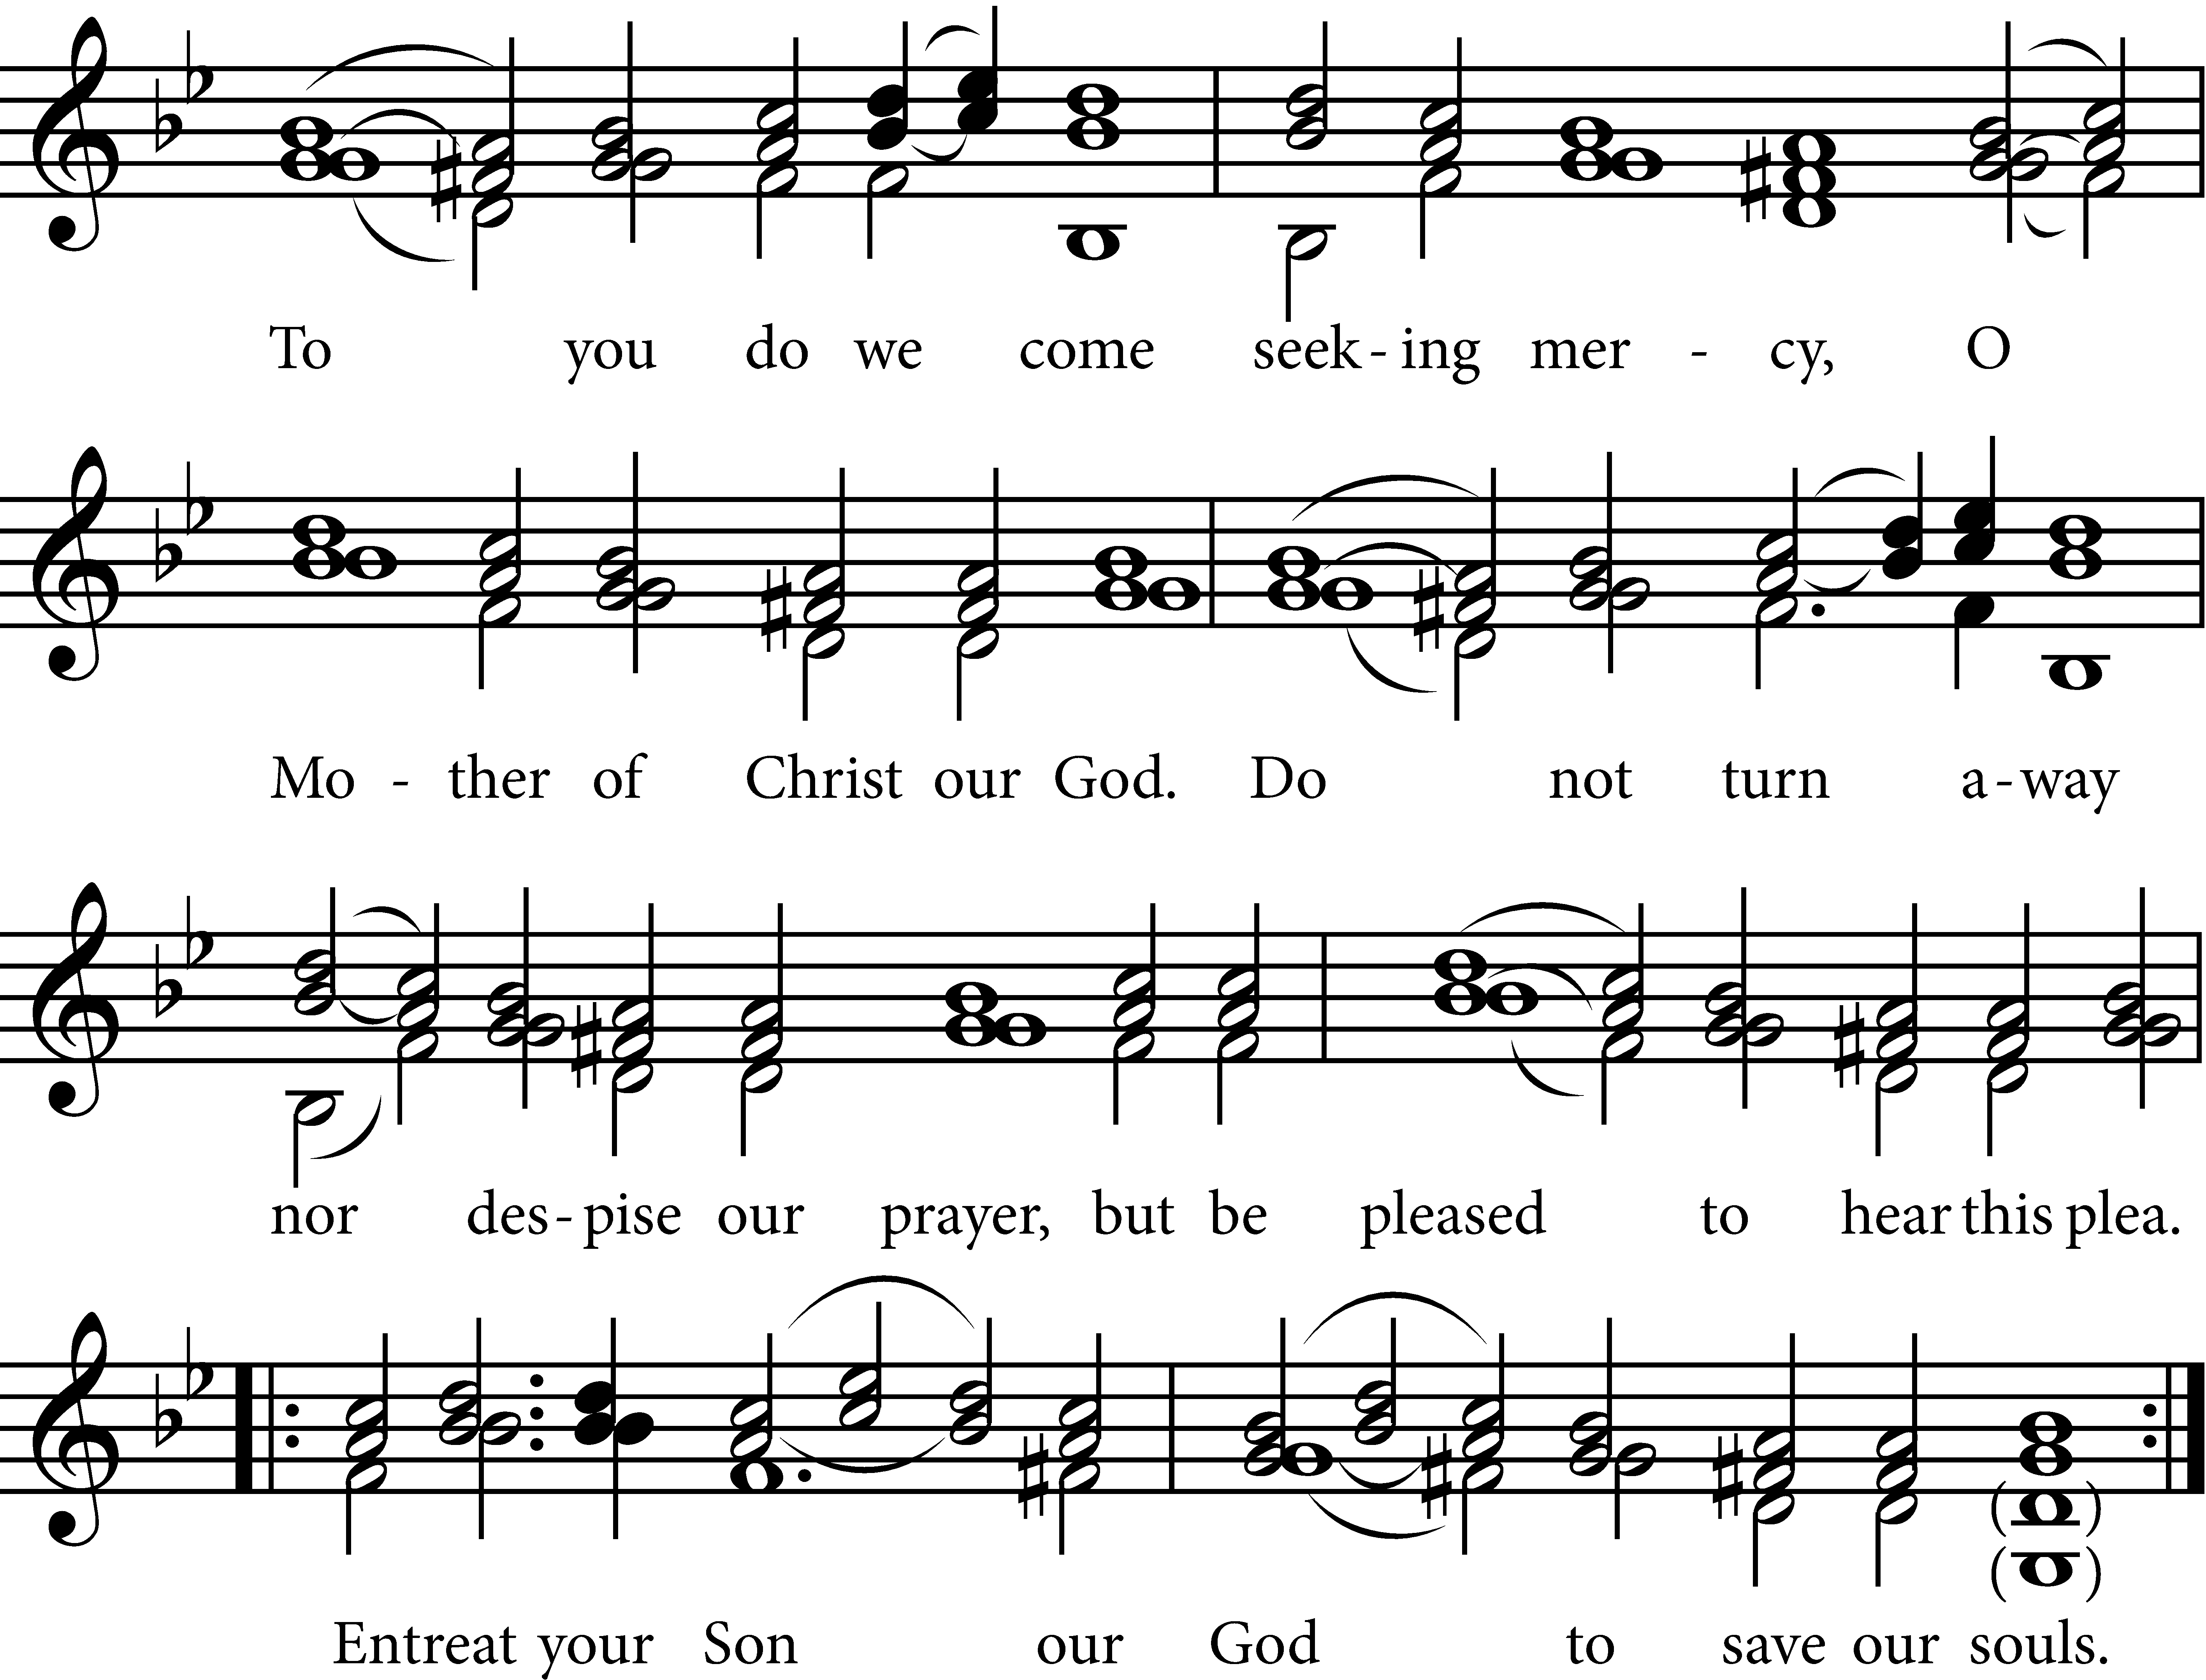
\includegraphics[width=\textwidth]{chants/an--sub_tuum--slavonic.png}\centering\end{figure}  \vspace{5pt} \emph{}  \newpage
\subsection{Advent}
 \subsubsection{Antiphona}  \greannotation{V} \index[Antiphona]{Alma Redemptoris (Solemn)} \label{Alma Redemptoris (Solemn) (Antiphona)} \grecommentary[5pt]{Ecclesia} \gresetinitiallines{1} \grechangestyle{initial}{\fontsize{36}{36}\selectfont} \grechangedim{maxbaroffsettextleft@nobar}{12 cm}{scalable} \grechangedim{spaceabovelines}{0.5cm}{scalable} \gresetlyriccentering{vowel}   \gregorioscore{chants/an--alma_redemptoris--solemn}  \vspace{5pt} \emph{Loving Mother of the Redeemer, you who remain the open gate of heaven, and the star of the sea, hasten to the aid of your people who, falling, strive to rise again. You who, to the wonderment of nature, bore your holy Creator, remaining a virgin after as before, receiving that ``Ave” from the mouth of Gabriel: have mercy on us sinners.}  \newpage
\subsection{Advent}
 \subsubsection{Antiphona}  \greannotation{V} \index[Antiphona]{Alma Redemptoris (Simple)} \label{Alma Redemptoris (Simple) (Antiphona)} \grecommentary[3pt]{Ecclesia} \gresetinitiallines{1} \grechangestyle{initial}{\fontsize{36}{36}\selectfont} \grechangedim{maxbaroffsettextleft@nobar}{12 cm}{scalable} \grechangedim{spaceabovelines}{0.5cm}{scalable} \gresetlyriccentering{vowel}   \gregorioscore{chants/an--alma_redemptoris--simple}  \vspace{5pt} \emph{ Loving Mother of the Redeemer, you who remain the open gate of heaven, and the star of the sea, hasten to the aid of your people who, falling, strive to rise again. You who, to the wonderment of nature, bore your holy Creator, remaining a virgin after as before, receiving that ``Ave” from the mouth of Gabriel: have mercy on us sinners.}  \newpage
\subsection{Lent}
 \subsubsection{Antiphona}  \greannotation{VI} \index[Antiphona]{Ave Regina cælorum (Solemn)} \label{Ave Regina cælorum (Solemn) (Antiphona)} \grecommentary[3pt]{Ecclesia} \gresetinitiallines{1} \grechangestyle{initial}{\fontsize{36}{36}\selectfont} \grechangedim{maxbaroffsettextleft@nobar}{12 cm}{scalable} \grechangedim{spaceabovelines}{0.5cm}{scalable} \gresetlyriccentering{vowel}   \gregorioscore{chants/an--ave_regina--solemn}  \vspace{5pt} \emph{Hail, Queen of Heaven. Hail, Mistress of the Angels. Hail the root, hail the gate, whence came the light of the world. Rejoice, O glorious Virgin, beautiful above all others. Farewell, O fairest one, and pray for us always to Christ.}  \newpage
\subsection{Lent}
 \subsubsection{Antiphona}  \greannotation{VI} \index[Antiphona]{Ave Regina cælorum (Simple)} \label{Ave Regina cælorum (Simple) (Antiphona)} \grecommentary[0pt]{Ecclesia} \gresetinitiallines{1} \grechangestyle{initial}{\fontsize{36}{36}\selectfont} \grechangedim{maxbaroffsettextleft@nobar}{12 cm}{scalable} \grechangedim{spaceabovelines}{0.5cm}{scalable} \gresetlyriccentering{vowel}   \gregorioscore{chants/an--ave_regina--simple}  \vspace{5pt} \emph{Hail, Queen of Heaven. Hail, Mistress of the Angels. Hail the root, hail the gate, whence came the light of the world. Rejoice, O glorious Virgin, beautiful above all others. Farewell, O fairest one, and pray for us always to Christ.}  \newpage
\subsection{Easter}
 \subsubsection{Antiphona}  \greannotation{VI} \index[Antiphona]{Regina cæli (Solemn)} \label{Regina cæli (Solemn) (Antiphona)} \grecommentary[0pt]{Ecclesia} \gresetinitiallines{1} \grechangestyle{initial}{\fontsize{36}{36}\selectfont} \grechangedim{maxbaroffsettextleft@nobar}{12 cm}{scalable} \grechangedim{spaceabovelines}{0.5cm}{scalable} \gresetlyriccentering{vowel}  \grechangestyle{translation}{\fontsize{11}{11}\selectfont} \gregorioscore{chants/an--regina_caeli--solemn} \grechangestyle{translation}{\fontsize{10}{10}\it\selectfont} \vspace{5pt} \emph{Queen of heaven, rejoice, alleluia. For he whom you were worthy to bear, alleluia, has risen (ascended) as he said, alleluia. Pray for us to God, alleluia.}  \newpage
\subsection{Easter}
 \subsubsection{Antiphona}  \greannotation{VI} \index[Antiphona]{Regina cæli (Simple)} \label{Regina cæli (Simple) (Antiphona)} \grecommentary[7pt]{Ecclesia} \gresetinitiallines{1} \grechangestyle{initial}{\fontsize{36}{36}\selectfont} \grechangedim{maxbaroffsettextleft@nobar}{12 cm}{scalable} \grechangedim{spaceabovelines}{0.5cm}{scalable} \gresetlyriccentering{vowel}  \grechangestyle{translation}{\fontsize{11}{11}\selectfont} \gregorioscore{chants/an--regina_caeli--simple} \grechangestyle{translation}{\fontsize{10}{10}\it\selectfont} \vspace{5pt} \emph{Queen of heaven, rejoice, alleluia. For he whom you were worthy to bear, alleluia, has risen (ascended) as he said, alleluia. Pray for us to God, alleluia.}  \newpage
\section{Chants in Honor of St. Dominic}
 \subsubsection{Responsorium prolixa}  \greannotation{I} \index[Responsorium prolixa]{O spem miram} \label{O spem miram (Responsorium prolixa)} \grecommentary[3pt]{Ecclesia} \gresetinitiallines{1} \grechangestyle{initial}{\fontsize{36}{36}\selectfont} \grechangedim{maxbaroffsettextleft@nobar}{12 cm}{scalable} \grechangedim{spaceabovelines}{0.45cm}{scalable} \gresetlyriccentering{vowel}   \gregorioscore{chants/rp--o_spem_miram--tp_et_non_tp}  \vspace{5pt} \emph{O wonderful hope, which you gave to those who wept for you at the hour of your death, promising that after your death you would be helpful to your brethren! * Fulfill, Father, what you have said, and help us by your prayers. \Vbar.~You shone on the bodies of the sick by so many miracles. Bring us the help of Christ to heal our sick souls. * Fulfill, Father, what you have said, and help us by your prayers.}
 \subsubsection{Antiphona}  \greannotation{I} \index[Antiphona]{Magne Pater} \label{Magne Pater (Antiphona)} \grecommentary[7pt]{Ecclesia} \gresetinitiallines{1} \grechangestyle{initial}{\fontsize{36}{36}\selectfont} \grechangedim{maxbaroffsettextleft@nobar}{12 cm}{scalable} \grechangedim{spaceabovelines}{0.5cm}{scalable} \gresetlyriccentering{vowel}   \gregorioscore{chants/an--magne_pater--compline}  \vspace{5pt} \emph{Great Father, holy Dominic, take us up with you at the hour of our death, and always watch over us lovingly here below.}
 \subsubsection{Antiphona}  \greannotation{I} \index[Antiphona]{Pie Pater} \label{Pie Pater (Antiphona)} \grecommentary[3pt]{Ecclesia} \gresetinitiallines{1} \grechangestyle{initial}{\fontsize{36}{36}\selectfont} \grechangedim{maxbaroffsettextleft@nobar}{12 cm}{scalable} \grechangedim{spaceabovelines}{0.5cm}{scalable} \gresetlyriccentering{vowel}   \gregorioscore{chants/an--pie_pater--compline}  \vspace{5pt} \emph{Great Father, holy Dominic, take us up with you at the hour of our death, and always watch over us lovingly here below.}



  \end{document}
